\chapter{生命世界的分类}\label{ch:b1:classifying-biodiversity}

已命名的\omterm{def:b1:classifying-biodiversity:species}{物种}约 200 万种，每年还会
新增约 \num{18000} 种；现存\omterm{def:b1:classifying-biodiversity:species}{物种}数估计接近
900 万种（仅真核生物一项），而细菌究竟
有多少种，无人知晓。命名只是开端：生物学家想知道的是
哪个\omterm{def:b1:classifying-biodiversity:species}{物种}与哪个\omterm{def:b1:classifying-biodiversity:species}{物种}最为亲近，答案是一棵树，因为
\omterm{def:b1:classifying-biodiversity:species}{物种}彼此通过世系相关联。本章介绍
命名规则，以及由\omterm{def:b1:classifying-biodiversity:characters}{性状}推断亲缘关系的方法——
以及用于判定竞争树优劣的标准，
即\omterm{def:b1:classifying-biodiversity:parsimony}{简约性}——生命之树目前所认识的形态，
以及现存生物清单的状况。

\section{物种与命名}

\begin{definition}[物种]\label{def:b1:classifying-biodiversity:species}
\index{物种}\index{生物学物种概念}
\emph{物种}依\emph{生物学物种概念}而言，是指一组
\omterm{def:b1:populations:population}{种群}，其成员能够相互交配并产生可育的
后代，且与其他此类群体存在生殖隔离。
该概念不能用于不进行有性生殖的生物，
即多数细菌、许多原生生物以及部分动植物，
也不能用于化石或从不相遇的\omterm{def:b1:populations:population}{种群}；此时物种
依其形态（\emph{形态学物种概念}）、
依其在树上独立的谱系（\emph{\omterm{def:b1:classifying-biodiversity:systematics}{系统发生}物种概念}），或
依遗传分化的阈值来\omterm{prop:b1:water-small-molecules:weak}{识别}。所有概念都试图指称
同一事物：与其他谱系分开、独立演化的谱系。
\end{definition}

\begin{definition}[命名法与分类阶元]\label{def:b1:classifying-biodiversity:nomenclature}
\index{双名法}\index{分类单元}\index{属}\index{模式标本}
每个\omterm{def:b1:classifying-biodiversity:species}{物种}都有一个\emph{双名法}名称：即其
\emph{属}名（首字母大写）后接种加词，两者都用
斜体——\emph{Homo sapiens}、\emph{Quercus robur}、
\emph{Escherichia coli}——通常还附有命名者与
描述年份。该体系由林奈于 1753 年（植物）和
1758 年（动物）确立，将\omterm{def:b1:classifying-biodiversity:species}{物种}嵌套于\emph{分类阶元}的层级中：属、
科、目、纲、门（植物学中称“门”）、界、域。
任一阶元上的群即为一个\emph{分类单元}。每个名称都与一个\emph{模式
标本}相连，该标本存放于博物馆或植物标本馆，用以确定此名称所指
的对象；最早的有效名称享有优先权；规则
经过编纂，使每个生物在全世界只有一个名称。分类阶元
只是约定——不存在所有科共有的属性，也没有哪一个
属具有这样的属性；只有\omterm{def:b1:classifying-biodiversity:species}{物种}才是自然单位。
\end{definition}

\begin{omfigure}
\begin{tikzpicture}[font=\footnotesize, line cap=round]
  \draw[thick, omDef!60!black, fill=omDef!6, rounded corners=4pt] (0,0) rectangle (11.4,5.4); \node[anchor=north west, omDef!80!black] at (0.1,5.35) {域 Eukarya};
  \draw[thick, omDef!60!black, fill=omDef!10, rounded corners=4pt] (0.4,0.3) rectangle (11.0,4.75); \node[anchor=north west, omDef!80!black] at (0.5,4.7) {界 Animalia};
  \draw[thick, omProp!70!black, fill=omProp!10, rounded corners=4pt] (0.8,0.6) rectangle (10.6,4.1); \node[anchor=north west, omProp!80!black] at (0.9,4.05) {门 Chordata};
  \draw[thick, omProp!70!black, fill=omProp!18, rounded corners=4pt] (1.2,0.9) rectangle (10.2,3.45); \node[anchor=north west, omProp!80!black] at (1.3,3.4) {纲 Mammalia};
  \draw[thick, omThm!70!black, fill=omThm!10, rounded corners=4pt] (1.6,1.2) rectangle (9.8,2.8); \node[anchor=north west, omThm!80!black] at (1.7,2.75) {目 Carnivora};
  \draw[thick, omThm!70!black, fill=omThm!20, rounded corners=4pt] (2.0,1.4) rectangle (5.6,2.3); \node[anchor=north west, omThm!80!black] at (2.1,2.25) {科 Felidae};
  \node[anchor=west] at (2.1,1.65) {属 \emph{Felis}：\emph{F.~catus}};
  \draw[thick, omThm!70!black, fill=omThm!20, rounded corners=4pt] (5.9,1.4) rectangle (9.5,2.3); \node[anchor=north west, omThm!80!black] at (6.0,2.25) {科 Canidae};
  \node[anchor=west] at (6.0,1.65) {属 \emph{Canis}：\emph{C.~lupus}};
\end{tikzpicture}

{\small 林奈分类体系中逐级嵌套的分类阶元，以猫和
狼为例。每个方框是一个\omterm{def:b1:classifying-biodiversity:nomenclature}{分类单元}；\omterm{def:b1:classifying-biodiversity:nomenclature}{双名法}给出属名和
种名。}
\end{omfigure}

\begin{omfigure}
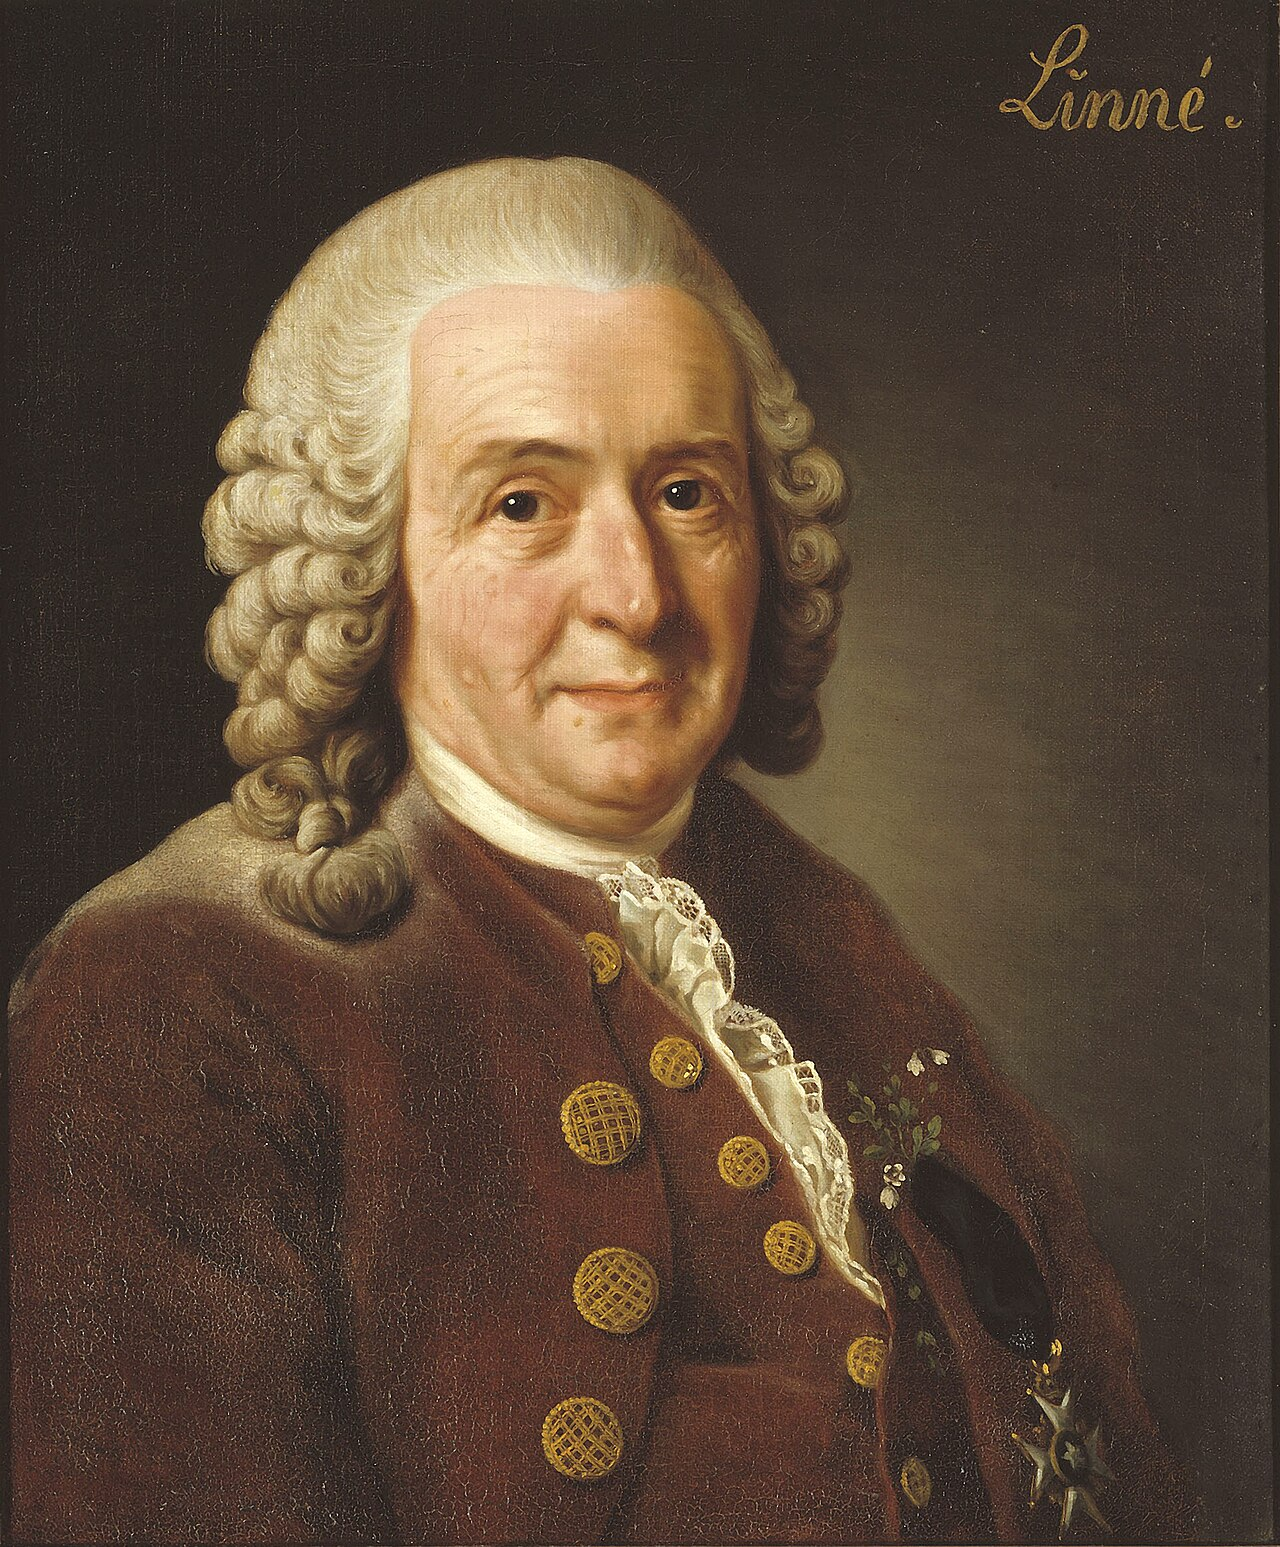
\includegraphics[width=0.36\linewidth]{images/book3/linnaeus.jpg}

{\small 卡尔·林奈（1707--1778），其 《植\omterm{def:b1:classifying-biodiversity:species}{物种}志》（1753 年）与
《自然系统》（1758 年第十版）是植物学与动物学命名的
起点。肖像
由亚历山大·罗斯林绘于 1775 年。}
\end{omfigure}

\begin{omfigure}
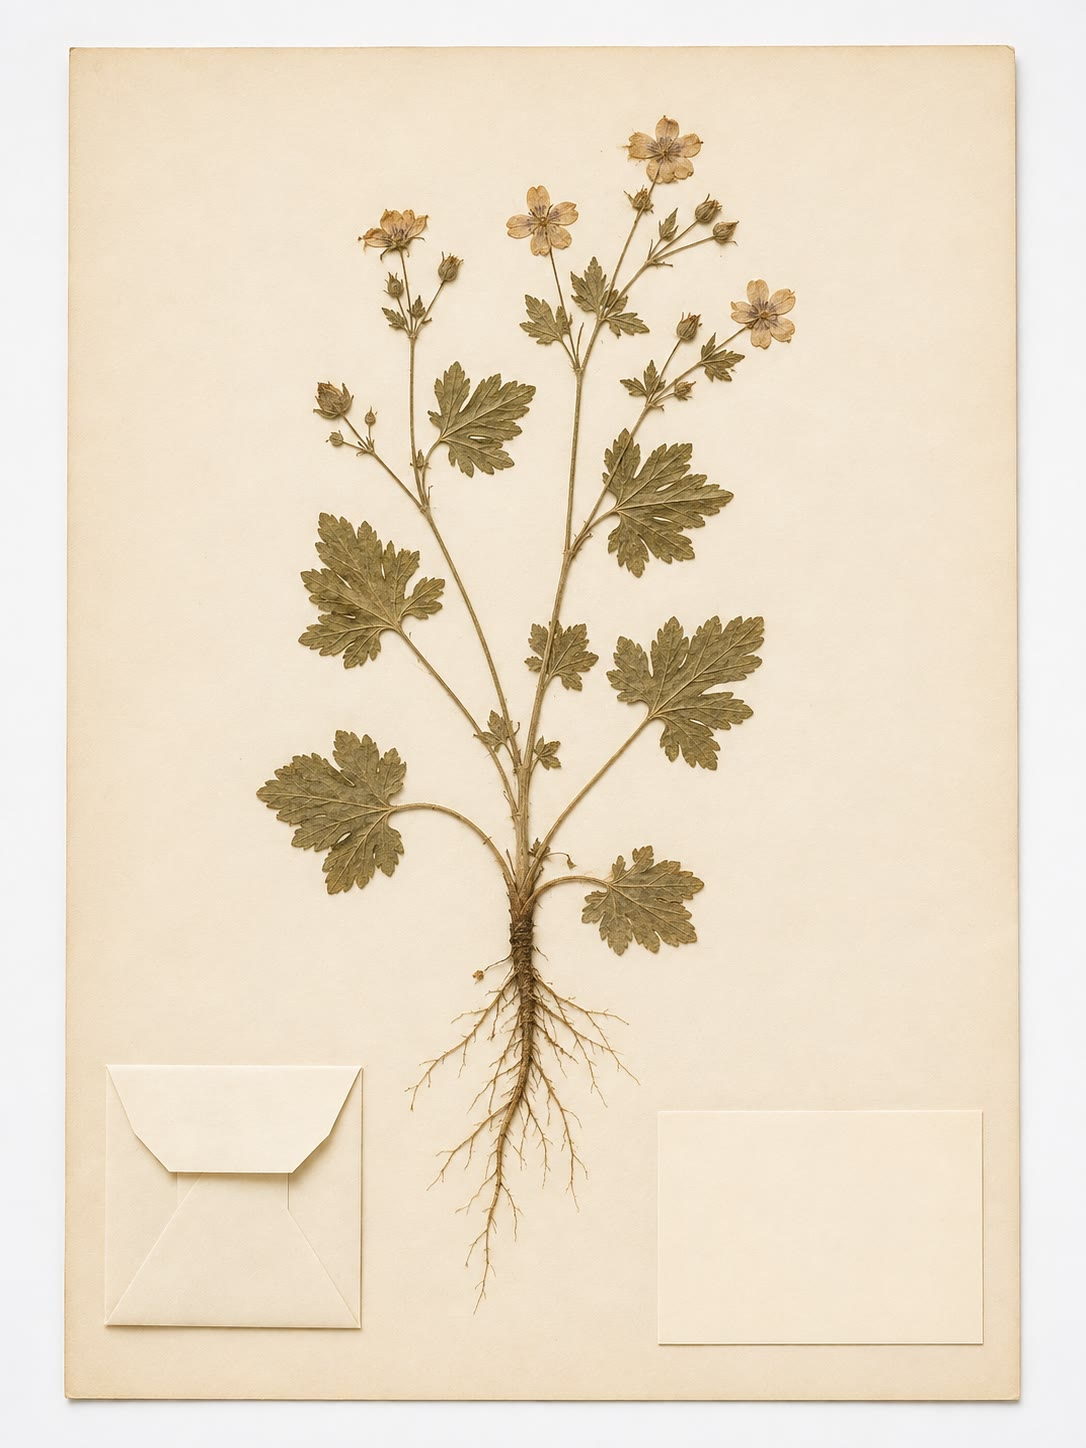
\includegraphics[width=0.5\linewidth]{images/book3/ai/b3-29-herbarium-sheet.jpg}

{\small 一幅植物标本纸页：压制并贴好标签的标本，
这类标本既可作为植物学名的模式，
也是\omterm{def:b1:classifying-biodiversity:species}{物种}采集地点和时间的永久凭证。}
\end{omfigure}

\section{重建亲缘关系}

\begin{definition}[系统学、系统发生与支序分类学]\label{def:b1:classifying-biodiversity:systematics}
\index{系统学}\index{系统发生}\index{支序分类学}\index{演化支}
\emph{系统学}研究生物的多样性及
它们之间的亲缘关系；\emph{系统发生}是这些关系的树，
即关于各谱系分化次序的假说。
\emph{表征分类学}按总体相似性为生物分组，平等计入所有
\omterm{def:b1:classifying-biodiversity:characters}{性状}；\emph{支序分类学}仅按共有衍生\omterm{def:b1:classifying-biodiversity:characters}{性状}分组，
使每个类群都是一个\emph{演化支}——一个祖先及其
全部后代。现代分类旨在使每个
已命名的\omterm{def:b1:classifying-biodiversity:nomenclature}{分类单元}都成为演化支。
\end{definition}

\begin{definition}[性状：同源、同塑与极性]\label{def:b1:classifying-biodiversity:characters}
\index{同源}\index{同塑}\index{共有衍征}\index{外群}
\emph{性状}是指任何具有两个或更多
\emph{状态}（如肢体有或无；某\omterm{def:b1:genomes:gene}{基因}中某一位点的碱基为 A、C、G
或 T）。两个生物的性状若来自共同祖先，则称为\emph{同源}的；
若因趋同或逆转而相似，则称为\emph{同塑}的，
（如鸟与蝙蝠的翅膀、海豚与鲨鱼的流线型身体）。
性状状态若在类群的祖先中已存在，则称为\emph{祖先的}
（祖征）；若在类群内部出现，则称为\emph{衍生的}
（衍征）；由一个\omterm{def:b1:classifying-biodiversity:systematics}{演化支}共有的衍生状态，即其\emph{共有衍征}，
是支持该\omterm{def:b1:classifying-biodiversity:systematics}{演化支}的唯一证据。
极性由与\emph{外群}相比较而确定，外群是一个
已知位于所研究类群之外的\omterm{def:b1:classifying-biodiversity:nomenclature}{分类单元}：其所示的状态
被视为祖先状态。
\end{definition}

\begin{definition}[单系、并系与多系]\label{def:b1:classifying-biodiversity:monophyly}
\index{单系}\index{并系}\index{多系}
若一个类群包含一个祖先及其全部后代，则称为\emph{单系}的（即\omterm{def:b1:classifying-biodiversity:systematics}{演化支}）；
若包含一个祖先及其部分后代，则称为\emph{并系}的
（如“爬行动物”，不包括由其演化而来的鸟类；
“鱼类”，不包括四足动物；“无脊椎动物”）；
若将由不同祖先演化而来的后代依趋同\omterm{def:b1:classifying-biodiversity:characters}{性状}归为一组，则称为\emph{多系}的
（如“温血动物”，即鸟类与哺乳动物；“藻类”）。并系类群可作为
\omterm{def:b1:body-plans-tissues:tissue}{组织}水平的有用描述，
但并非\omterm{def:b1:classifying-biodiversity:systematics}{演化支}，
且已不再给予正式名称。
\end{definition}

\begin{omfigure}
\begin{tikzpicture}[font=\footnotesize, line cap=round, >=Stealth]
  % tree: lamprey, shark, trout, lungfish, frog, lizard, bird, mammal
  \coordinate (r) at (6.5,-1.2);
  \draw[thick] (r) -- (6.5,-0.2);
  \draw[thick] (6.5,-0.2) -- (0.5,-0.2) -- (0.5,4.6); \node[anchor=south, rotate=60, anchor=west] at (0.5,4.6) {七鳃鳗};
  \draw[thick] (6.5,-0.2) -- (6.5,0.6) -- (2.2,0.6) -- (2.2,4.6); \node[rotate=60, anchor=west] at (2.2,4.6) {鲨鱼};
  \draw[thick] (6.5,0.6) -- (6.5,1.3) -- (3.8,1.3) -- (3.8,4.6); \node[rotate=60, anchor=west] at (3.8,4.6) {鳟鱼};
  \draw[thick] (6.5,1.3) -- (6.5,2.0) -- (5.2,2.0) -- (5.2,4.6); \node[rotate=60, anchor=west] at (5.2,4.6) {肺鱼};
  \draw[thick] (6.5,2.0) -- (6.5,2.7) -- (6.6,2.7) -- (6.6,4.6); \node[rotate=60, anchor=west] at (6.6,4.6) {青蛙};
  \draw[thick] (6.5,2.7) -- (8.7,2.7) -- (8.7,3.3);
  \draw[thick] (8.7,3.3) -- (8.0,3.3) -- (8.0,4.6); \node[rotate=60, anchor=west] at (8.0,4.6) {哺乳动物};
  \draw[thick] (8.7,3.3) -- (9.7,3.3) -- (9.7,3.9);
  \draw[thick] (9.7,3.9) -- (9.3,3.9) -- (9.3,4.6); \node[rotate=60, anchor=west] at (9.3,4.6) {蜥蜴};
  \draw[thick] (9.7,3.9) -- (10.6,3.9) -- (10.6,4.6); \node[rotate=60, anchor=west] at (10.6,4.6) {鸟};
  % groupings
  \draw[very thick, omDef, rounded corners=6pt] (7.6,3.05) rectangle (11.0,5.9); \node[omDef!80!black, anchor=south west] at (7.65,5.9) {羊膜动物：单系};
  \draw[very thick, omThm, dashed, rounded corners=6pt] (9.0,3.6) -- (9.0,5.8) -- (10.15,5.8) -- (10.15,3.6) -- cycle; \node[omThm!80!black, anchor=west, align=left] at (11.1,4.8) {“爬行动物”\\ 不含鸟类：\\ 并系};
  \draw[very thick, omProp!80!black, dotted, rounded corners=6pt] (7.7,6.35) -- (7.7,6.8) -- (11.0,6.8) -- (11.0,6.35); \node[omProp!80!black, anchor=south] at (9.35,6.85) {“温血动物”（哺乳动物 $+$ 鸟类）：多系};
  \draw[very thick, gray, dashed, rounded corners=6pt] (1.8,4.3) -- (1.8,5.75) -- (5.7,5.75) -- (5.7,4.3); \node[gray, anchor=south] at (3.75,5.9) {“鱼类”不含四足动物：并系};
  % synapomorphies
  \node[font=\scriptsize, anchor=east] at (6.4,0.2) {颌}; \draw[thick] (6.35,0.2) -- (6.65,0.2);
  \node[font=\scriptsize, anchor=east] at (6.4,0.95) {硬骨骼}; \draw[thick] (6.35,0.95) -- (6.65,0.95);
  \node[font=\scriptsize, anchor=east] at (6.4,1.65) {肺}; \draw[thick] (6.35,1.65) -- (6.65,1.65);
  \node[font=\scriptsize, anchor=east] at (6.4,2.35) {四肢}; \draw[thick] (6.35,2.35) -- (6.65,2.35);
  \node[font=\scriptsize, anchor=west] at (8.8,2.82) {羊膜卵}; \draw[thick] (8.55,2.82) -- (8.85,2.82);
\end{tikzpicture}

{\small 八种脊椎动物的分支图，分支上标出了
\omterm{def:b1:classifying-biodiversity:characters}{共有衍征}。\omterm{def:b1:classifying-biodiversity:systematics}{演化支}均为\omterm{def:b1:classifying-biodiversity:monophyly}{单系}；“鱼类”与“爬行动物”
为\omterm{def:b1:classifying-biodiversity:monophyly}{并系}类群，“温血动物”则是依趋同\omterm{def:b1:classifying-biodiversity:characters}{性状}划分的
\omterm{def:b1:classifying-biodiversity:monophyly}{多系}类群。}
\end{omfigure}

\begin{definition}[简约性]\label{def:b1:classifying-biodiversity:parsimony}
\index{简约性}\index{树长}
在所有能够联系一组\omterm{def:b1:classifying-biodiversity:nomenclature}{分类单元}的树中，\emph{最简约}的
树是所需\omterm{def:b1:classifying-biodiversity:characters}{性状}状态演化变化最少的那一棵——
即\emph{树长}最小者，树长为各\omterm{def:b1:classifying-biodiversity:characters}{性状}在该树上所需
的最少变化次数之和。若某\omterm{def:b1:classifying-biodiversity:characters}{性状}在该树上只需一次变化，
则称其与该树相容；若需两次或更多变化，则称其在该树上为\omterm{def:b1:classifying-biodiversity:characters}{同塑}\omterm{def:b1:classifying-biodiversity:characters}{性状}。
简约性并非断言演化是经济的；
它是一条规则：假说不应
引入多于数据所要求的
趋同现象。
\end{definition}

\begin{method}[由性状矩阵构建分支图]\label{met:b1:classifying-biodiversity:cladogram}
\begin{enumerate}
  \item 选定\omterm{def:b1:classifying-biodiversity:nomenclature}{分类单元}与\omterm{def:b1:classifying-biodiversity:characters}{外群}，列出各\omterm{def:b1:classifying-biodiversity:characters}{性状}及其
        状态，将\omterm{def:b1:classifying-biodiversity:characters}{外群}的状态编码为 0（祖先的），
        衍生状态编码为 1。
  \item 依共有衍生状态对\omterm{def:b1:classifying-biodiversity:nomenclature}{分类单元}分组，
        从最多\omterm{def:b1:classifying-biodiversity:nomenclature}{分类单元}共有的\omterm{def:b1:classifying-biodiversity:characters}{性状}（最深的\omterm{def:b1:classifying-biodiversity:systematics}{演化支}）起步，
        逐层向内嵌套；每个由一组\omterm{def:b1:classifying-biodiversity:nomenclature}{分类单元}共有的 1，
        都是该组的候选\omterm{def:b1:classifying-biodiversity:characters}{共有衍征}。
  \item 若\omterm{def:b1:classifying-biodiversity:characters}{性状}相互冲突（两种分组不能同时为
        \omterm{def:b1:classifying-biodiversity:systematics}{演化支}），则画出每一种备选树并计算其\omterm{def:b1:classifying-biodiversity:parsimony}{树长}：
        对每个\omterm{def:b1:classifying-biodiversity:characters}{性状}，取将其状态置于该树上所需的
        最少变化次数。
  \item 保留最短的树；在该树上需额外变化的
        \omterm{def:b1:classifying-biodiversity:characters}{性状}即为\omterm{def:b1:classifying-biodiversity:characters}{同塑}\omterm{def:b1:classifying-biodiversity:characters}{性状}。若两棵树等长，则
        数据无法作出判定，需要更多\omterm{def:b1:classifying-biodiversity:characters}{性状}。
  \item 阅读该树：为各\omterm{def:b1:classifying-biodiversity:systematics}{演化支}命名，指出哪些传统
        类群为\omterm{def:b1:classifying-biodiversity:monophyly}{并系}，并核对其是否与独立数据
        （分子序列、化石）相符。
\end{enumerate}
\end{method}

\begin{example}[两棵树，逐一计数]\label{ex:b1:classifying-biodiversity:count}
四个\omterm{def:b1:classifying-biodiversity:nomenclature}{分类单元}：蜥蜴、鸟、哺乳动物、青蛙（\omterm{def:b1:classifying-biodiversity:characters}{外群}）。\omterm{def:b1:classifying-biodiversity:characters}{性状}：
羊膜卵（蜥蜴、鸟、哺乳动物：1）、双孔型颅骨（蜥蜴、
鸟）、恒温性（鸟、哺乳动物）。树 A：先（蜥蜴，鸟），再与哺乳动物相接：
羊膜卵 1 次变化，颅骨 1 次，恒温性 2 次（独立出现两次）——\omterm{def:b1:classifying-biodiversity:parsimony}{树长} 4。
树 B：先（鸟，哺乳动物），再与蜥蜴相接：羊膜卵 1 次，恒温性 1 次，颅骨 2 次——
\omterm{def:b1:classifying-biodiversity:parsimony}{树长} 4。二者相等；再加入羽毛以及腿部鳞片与\omterm{def:b1:flowering-plant-organization:tissues}{表皮}鳞片
（蜥蜴、鸟）：树 A \omterm{def:b1:classifying-biodiversity:parsimony}{树长} 5，树 B \omterm{def:b1:classifying-biodiversity:parsimony}{树长} 6。树 A 更优，
且恒温性是\omterm{def:b1:classifying-biodiversity:characters}{同塑}\omterm{def:b1:classifying-biodiversity:characters}{性状}：它独立演化了两次。
\end{example}

\begin{omfigure}
\begin{tikzpicture}[font=\footnotesize, line cap=round]
  \begin{scope}
    \draw[thick] (2.0,0) -- (2.0,0.8);
    \draw[thick] (2.0,0.8) -- (0,0.8) -- (0,3.0); \node[anchor=south] at (0,3.0) {青蛙};
    \draw[thick] (2.0,0.8) -- (2.0,1.6) -- (1.2,1.6) -- (1.2,3.0); \node[anchor=south] at (1.2,3.0) {哺乳动物};
    \draw[thick] (2.0,1.6) -- (3.0,1.6) -- (3.0,2.3);
    \draw[thick] (3.0,2.3) -- (2.4,2.3) -- (2.4,3.0); \node[anchor=south] at (2.4,3.0) {蜥蜴};
    \draw[thick] (3.0,2.3) -- (3.6,2.3) -- (3.6,3.0); \node[anchor=south] at (3.6,3.0) {鸟};
    \draw[very thick, omDef] (1.85,1.2) -- (2.15,1.2); \node[anchor=east, font=\scriptsize, omDef!80!black] at (1.8,1.2) {羊膜卵};
    \draw[very thick, omDef] (2.85,1.95) -- (3.15,1.95); \node[anchor=west, font=\scriptsize, omDef!80!black] at (3.2,1.95) {颅骨、鳞片};
    \draw[very thick, omThm] (1.05,2.5) -- (1.35,2.5); \node[anchor=east, font=\scriptsize, omThm] at (1.0,2.5) {恒温};
    \draw[very thick, omThm] (3.45,2.65) -- (3.75,2.65); \node[anchor=west, font=\scriptsize, omThm] at (3.8,2.65) {恒温};
    \node[anchor=north, align=center] at (1.9,-0.2) {树 A：树长 5\\ （恒温性出现两次）};
  \end{scope}
  \begin{scope}[xshift=7.4cm]
    \draw[thick] (2.0,0) -- (2.0,0.8);
    \draw[thick] (2.0,0.8) -- (0,0.8) -- (0,3.0); \node[anchor=south] at (0,3.0) {青蛙};
    \draw[thick] (2.0,0.8) -- (2.0,1.6) -- (1.2,1.6) -- (1.2,3.0); \node[anchor=south] at (1.2,3.0) {蜥蜴};
    \draw[thick] (2.0,1.6) -- (3.0,1.6) -- (3.0,2.3);
    \draw[thick] (3.0,2.3) -- (2.4,2.3) -- (2.4,3.0); \node[anchor=south] at (2.4,3.0) {哺乳动物};
    \draw[thick] (3.0,2.3) -- (3.6,2.3) -- (3.6,3.0); \node[anchor=south] at (3.6,3.0) {鸟};
    \draw[very thick, omDef] (1.85,1.2) -- (2.15,1.2); \node[anchor=east, font=\scriptsize, omDef!80!black] at (1.8,1.2) {羊膜卵};
    \draw[very thick, omDef] (2.85,1.95) -- (3.15,1.95); \node[anchor=west, font=\scriptsize, omDef!80!black] at (3.2,1.95) {恒温};
    \draw[very thick, omThm] (1.05,2.5) -- (1.35,2.5); \node[anchor=east, font=\scriptsize, omThm, align=right] at (1.0,2.5) {颅骨、\\ 鳞片};
    \draw[very thick, omThm] (3.45,2.65) -- (3.75,2.65); \node[anchor=west, font=\scriptsize, omThm, align=left] at (3.8,2.65) {颅骨、\\ 鳞片};
    \node[anchor=north, align=center] at (1.9,-0.2) {树 B：树长 6\\ （颅骨与鳞片各出现两次）};
  \end{scope}
\end{tikzpicture}

{\small 简约法比较两棵树各自所需的变化数，
树 A 需要一次\omterm{def:b1:classifying-biodiversity:characters}{同塑}性（恒温性独立出现两次）；
树 B 需要两次；保留树 A。}
\end{omfigure}

\begin{remark}[分子性状]\label{rem:b1:classifying-biodiversity:molecular}
一段\omterm{def:b1:genomes:gene}{基因}序列一次即可提供数百个\omterm{def:b1:classifying-biodiversity:characters}{性状}，每个位点都是一个
具有四种状态的\omterm{def:b1:classifying-biodiversity:characters}{性状}，可用于比较那些没有任何可见共同特征的生物，
例如细菌与橡树。序列经比对后，\omterm{def:b1:classifying-biodiversity:characters}{同源}位点逐一相互比较，
再通过简约法或统计方法构建树；
统计方法对替换速率进行建模。分子钟即中性差异积累的速率，
用于推定分化的时间。这些方法，以及
长枝与速率不等所带来的陷阱，
将在本科二年级分册中讨论。
\end{remark}

\section{生命之树}

\begin{proposition}[三域]\label{prop:b1:classifying-biodiversity:domains}
\index{域}\index{古菌域}\index{细菌域}\index{真核域}
生命分为三域：\emph{细菌域}、\emph{古菌域} 和
\emph{真核域}。细菌与古菌的\omterm{def:b1:cell-unit-of-life:cell}{细胞}\omterm{def:b1:body-plans-tissues:tissue}{组织}均为原\omterm{def:b1:genomes:karyotype}{核型}（见
\cref{ch:b1:cell-unit-of-life}），但二者在膜脂、\omterm{def:b1:eukaryotic-cell:plantcell}{细胞壁}、\omterm{def:b1:nucleic-acids:chain}{RNA} 聚合酶
和\omterm{def:b1:gene-expression:ribosome}{核糖体}上有所不同；古菌的转录与翻译机制
比细菌更接近真核生物，\omterm{def:b1:cell-unit-of-life:prokeuk}{真核细胞}起源于
一支古菌谱系，该谱系吸收了一个细菌
作为其\omterm{def:b1:eukaryotic-cell:mitochondrion}{线粒体}（见\cref{ch:b1:eukaryotic-cell}）。在真核生物内部，
传统的“界”——动物、植物、真菌及一个“原生生物”剩余类——
被少数几个主要谱系取代，其中动物、真菌
与陆生植物只是三根小枝，
而“原生生物”则是其余一切的
\omterm{def:b1:classifying-biodiversity:monophyly}{并系}集合。
\end{proposition}
\begin{proof}[证据]
沃斯与福克斯（1977）比较了小亚基
\omterm{def:b1:gene-expression:ribosome}{核糖体} \omterm{def:b1:nucleic-acids:chain}{RNA} 的序列——这种分子每个\omterm{def:b1:cell-unit-of-life:cell}{细胞}都有，功能相同，
且在整个生命世界中可以比对——对细菌、产甲烷菌和
真核生物进行比较，发现产甲烷菌与其他细菌的差异，
与其和真核生物的差异一样大。原核生物由此分为两类，
而非一类；仅由这一\omterm{def:b1:genomes:gene}{基因}构建的树，
已被全\omterm{def:b1:genomes:genome}{基因组}数据及古菌独特的生物化学所证实，
即醚键相连的脂质且不含\omterm{def:b1:carbohydrates:polysaccharide}{肽聚糖}。
\end{proof}

\begin{omfigure}
\begin{tikzpicture}[font=\footnotesize, line cap=round]
  \coordinate (root) at (5.0,0);
  \draw[very thick] (root) -- (5.0,1.0);
  \draw[very thick, omExo!80!black] (5.0,1.0) -- (1.6,1.0) -- (1.6,2.4);
  \draw[very thick, omExo!80!black] (1.6,2.4) -- (0.4,2.4) -- (0.4,3.6); \draw[very thick, omExo!80!black] (1.6,2.4) -- (1.6,3.6); \draw[very thick, omExo!80!black] (1.6,2.4) -- (2.8,2.4) -- (2.8,3.6);
  \node[anchor=south, rotate=60, anchor=west] at (0.4,3.6) {变形菌门}; \node[rotate=60, anchor=west] at (1.6,3.6) {蓝细菌}; \node[rotate=60, anchor=west] at (2.8,3.6) {格拉姆阳性菌};
  \node[omExo!80!black, font=\small, anchor=north] at (1.6,0.9) {细菌};
  \draw[very thick] (5.0,1.0) -- (7.6,1.0) -- (7.6,1.7);
  \draw[very thick, omProp!80!black] (7.6,1.7) -- (5.8,1.7) -- (5.8,2.4);
  \draw[very thick, omProp!80!black] (5.8,2.4) -- (5.0,2.4) -- (5.0,3.6); \draw[very thick, omProp!80!black] (5.8,2.4) -- (6.6,2.4) -- (6.6,3.6);
  \node[rotate=60, anchor=west] at (5.0,3.6) {产甲烷菌}; \node[rotate=60, anchor=west] at (6.6,3.6) {嗜盐菌};
  \node[omProp!80!black, font=\small, anchor=north] at (5.8,1.6) {古菌};
  \draw[very thick, omDef] (7.6,1.7) -- (9.6,1.7) -- (9.6,2.4);
  \draw[very thick, omDef] (9.6,2.4) -- (8.0,2.4) -- (8.0,3.6); \draw[very thick, omDef] (9.6,2.4) -- (9.0,2.4) -- (9.0,3.6); \draw[very thick, omDef] (9.6,2.4) -- (10.0,2.4) -- (10.0,3.6); \draw[very thick, omDef] (9.6,2.4) -- (11.0,2.4) -- (11.0,3.6);
  \node[rotate=60, anchor=west] at (8.0,3.6) {陆生植物、藻类}; \node[rotate=60, anchor=west] at (9.0,3.6) {真菌}; \node[rotate=60, anchor=west] at (10.0,3.6) {动物}; \node[rotate=60, anchor=west] at (11.0,3.6) {许多原生生物谱系};
  \node[omDef!80!black, font=\small, anchor=north] at (9.6,1.6) {真核生物};
  \draw[->, thick, gray, dashed] (1.6,2.0) to[out=0, in=180] (9.6,2.1); \node[gray, font=\scriptsize, anchor=west] at (5.2,0.5) {一个细菌成为线粒体};
  \node[anchor=north] at (5.0,-0.1) {末次通用共同祖先};
\end{tikzpicture}

{\small 三域，依据\omterm{def:b1:gene-expression:ribosome}{核糖体} \omterm{def:b1:nucleic-acids:chain}{RNA} 绘制。古菌与真核生物
亲缘关系更近，\omterm{def:b1:cell-unit-of-life:prokeuk}{真核细胞}是一种融合体：
以古菌为宿主、以细菌为\omterm{def:b1:eukaryotic-cell:mitochondrion}{线粒体}（在植物和
藻类中，还有第二个细菌伙伴，即\omterm{def:b1:photosynthesis:chloroplast}{叶绿体}）。}
\end{omfigure}

\begin{omfigure}
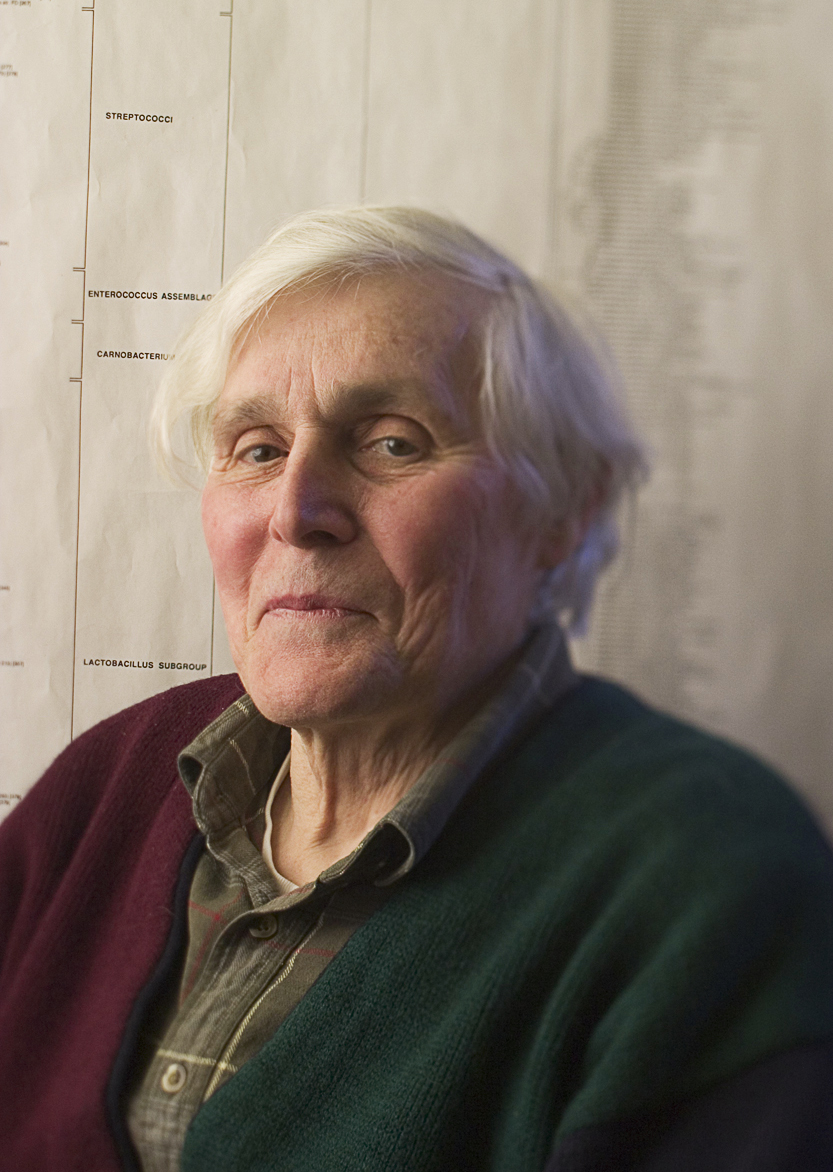
\includegraphics[width=0.34\linewidth]{images/book3/woese.jpg}

{\small 卡尔·沃斯（1928--2012）站在一棵基于\omterm{def:b1:gene-expression:ribosome}{核糖体} \omterm{def:b1:nucleic-acids:chain}{RNA} 的
细菌树前。他对这一分子在整个生命世界中的比较，
揭示了古菌，并使生命之树有了三域之分。}
\end{omfigure}

\begin{proposition}[真核生物的主要谱系]\label{prop:b1:classifying-biodiversity:eukaryotes}
真核生物可分为几大类群：\emph{后鞭毛生物}
（动物、真菌及其单\omterm{def:b1:cell-unit-of-life:cell}{细胞}近亲，其\omterm{def:b1:cell-unit-of-life:cell}{细胞}以后端一根鞭毛游动）；
\emph{Archaeplastida}（陆生植物、绿藻与红藻，具初生\omterm{def:b1:photosynthesis:chloroplast}{叶绿体}）；
\emph{Amoebozoa}；\emph{Excavata}（鞭毛虫，如
\emph{Trypanosoma} 与 \emph{Euglena}）；\emph{SAR} 类群
（不等鞭毛类，如硅藻与褐藻；囊泡虫类，如纤毛虫、
甲藻与疟原虫；根足类，如
有孔虫与放射虫）。因此，动物与真菌彼此的
亲缘关系比二者中任一与植物的都更近；“藻类”
分散于四个类群之中；而真核\omterm{def:b1:classifying-biodiversity:biodiversity}{生物多样性}中
绝大多数微小的成员，
都位于三个有常用名的界之外。
\end{proposition}

\begin{omfigure}
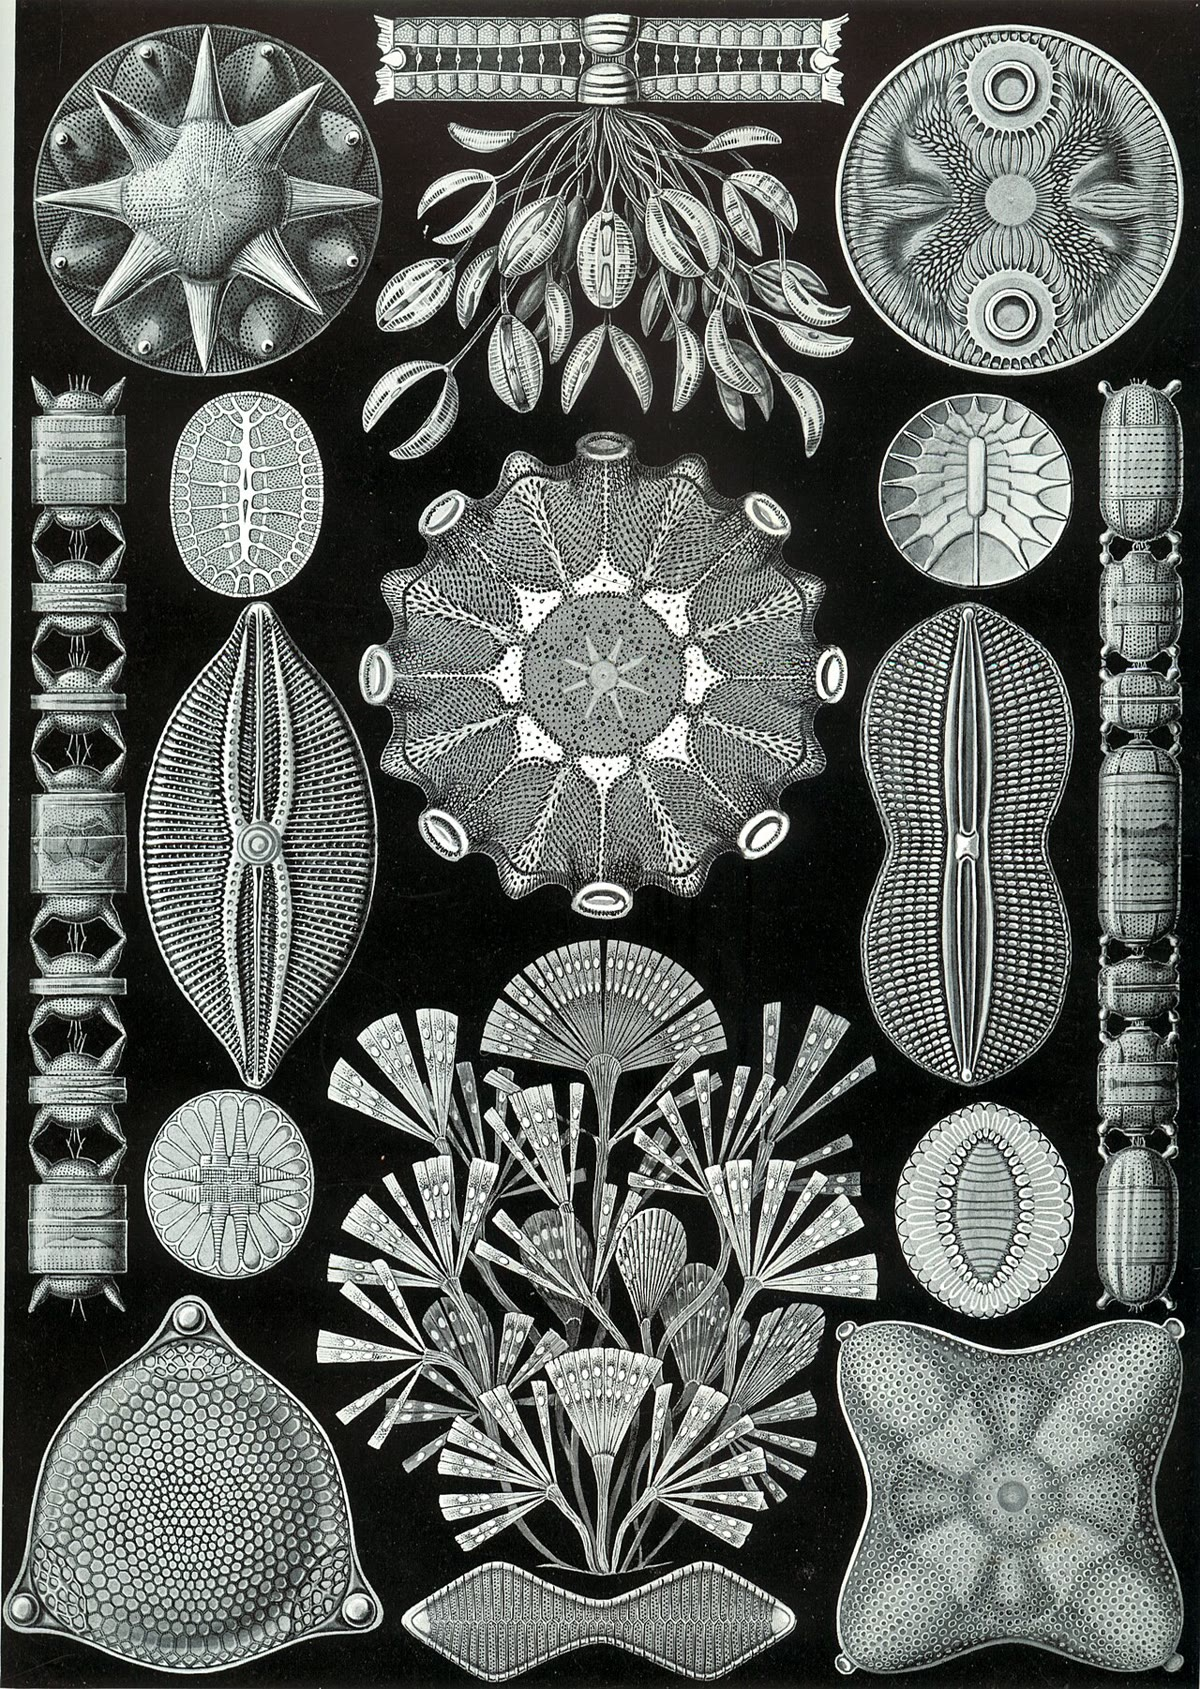
\includegraphics[width=0.36\linewidth]{images/book3/haeckel-diatomea.jpg}\hspace{0.03\linewidth}
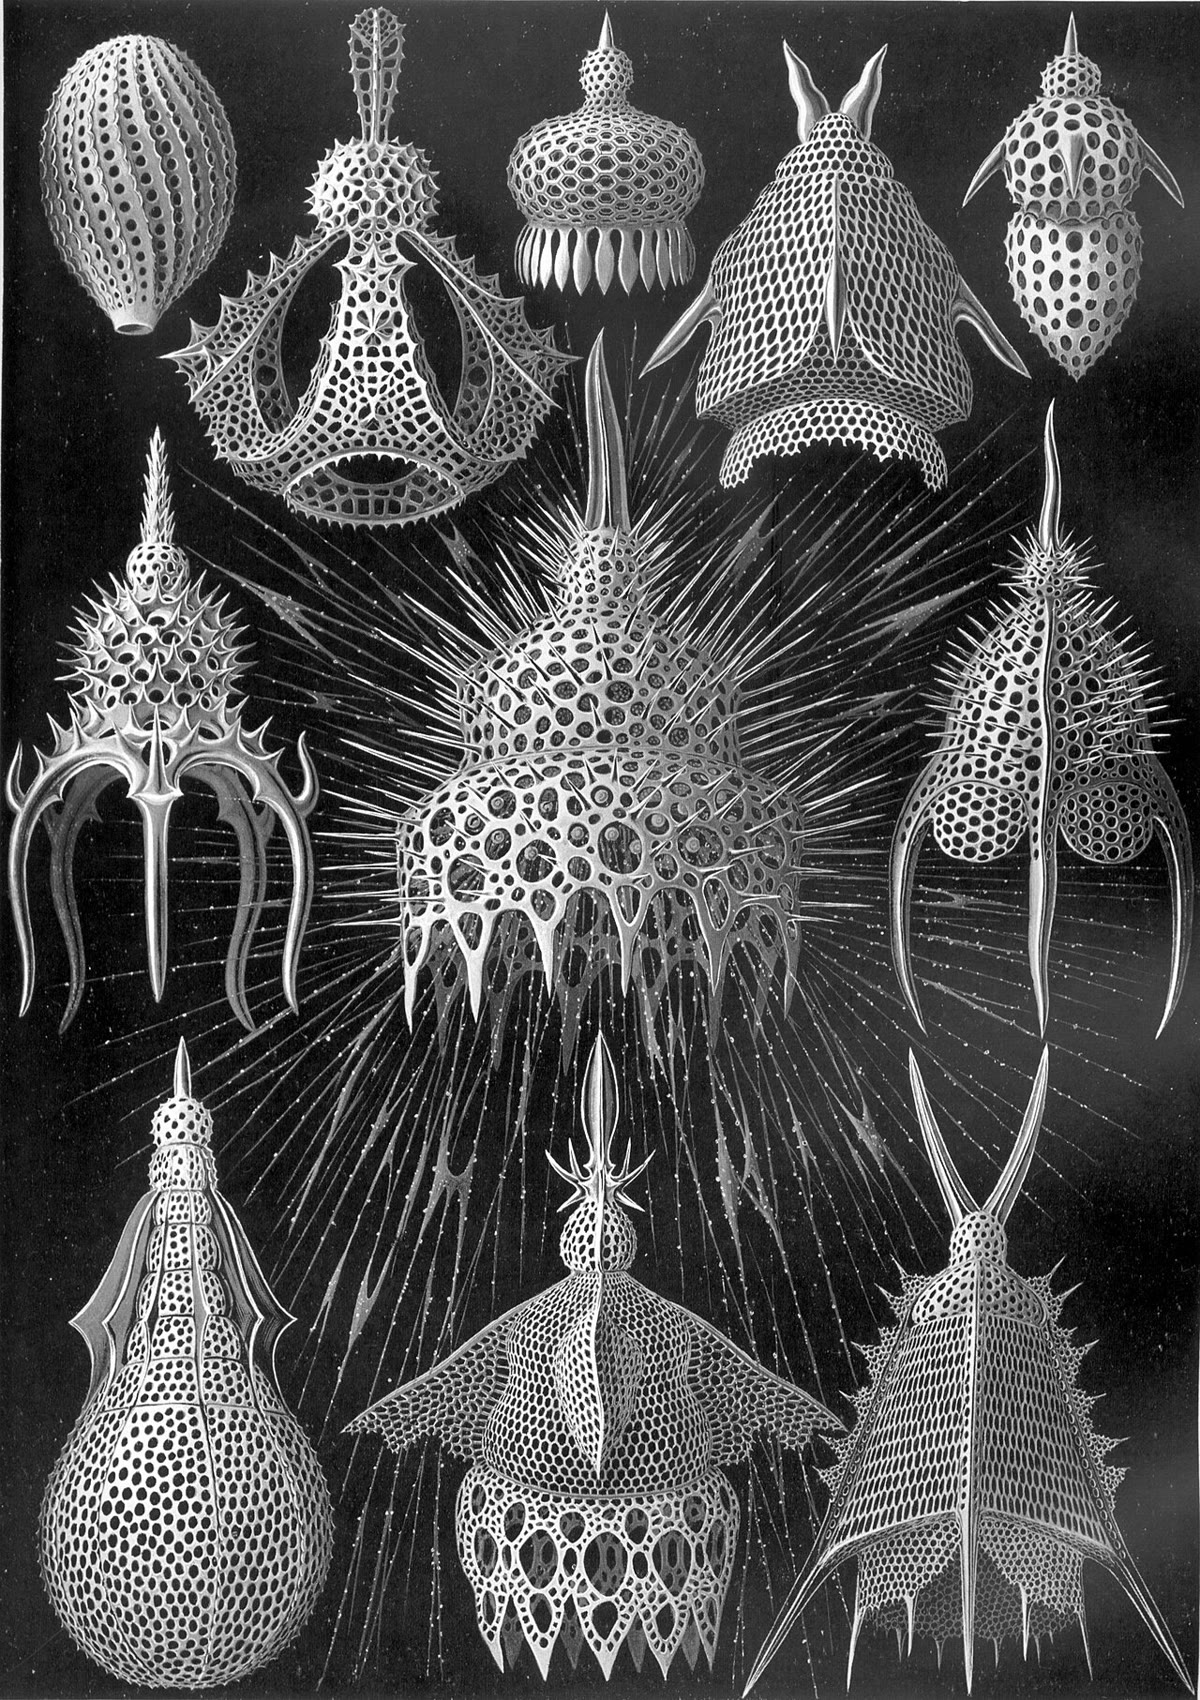
\includegraphics[width=0.36\linewidth]{images/book3/haeckel-cyrtoidea.jpg}

{\small 两个没有常用名的真核生物谱系，
取自恩斯特·海克尔 1904 年的图版：硅藻（不等鞭毛类，
硅质壳体）与放射虫（根足类，硅质\omterm{def:b1:body-plans-tissues:segments}{骨骼}）。每一
类群都包含数以万计的\omterm{def:b1:classifying-biodiversity:species}{物种}。}
\end{omfigure}

\section{生命的清单}

\begin{definition}[生物多样性]\label{def:b1:classifying-biodiversity:biodiversity}
\index{生物多样性}\index{灭绝}
\emph{生物多样性}是各个层次上的生命多样性：\omterm{def:b1:classifying-biodiversity:species}{物种}内的遗传
多样性、\omterm{def:b1:classifying-biodiversity:species}{物种}的数量与丰度，
以及\omterm{def:b1:ecosystem-organization:ecosystem}{群落}与\omterm{def:b1:ecosystem-organization:ecosystem}{生态系统}的多样性。其清单尚未完成：
约 200 万种\omterm{def:b1:classifying-biodiversity:species}{物种}已被描述，其中一百万为昆虫，
\num{380000} 种植物，\num{150000} 种真菌，
\num{70000} 种脊椎动物，以及软体动物、甲壳动物、
原生生物和原核生物各有数万种；真核生物\omterm{def:b1:classifying-biodiversity:species}{物种}的数量
依据新高级\omterm{def:b1:classifying-biodiversity:nomenclature}{分类单元}仍在不断被发现的速率估算，
约接近 900 万种，因此多数\omterm{def:b1:classifying-biodiversity:species}{物种}尚未命名，
而其中大多数体型微小、生活于热带，或二者兼具。
\omterm{def:b1:classifying-biodiversity:species}{物种}一直在\emph{灭绝}：据化石推算，背景速率约为
每百万\omterm{def:b1:classifying-biodiversity:species}{物种}每年一种，而当前速率由\omterm{def:b1:ecosystem-organization:niche}{栖息地}丧失、过度利用、
入侵\omterm{def:b1:classifying-biodiversity:species}{物种}与气候变化所驱动，估计为背景速率的
一百至一千倍。
\end{definition}

\begin{omfigure}
\begin{tikzpicture}
\begin{axis}[
  xbar, bar width=7pt,
  width=0.82\linewidth, height=6.8cm,
  axis x line=bottom, axis y line=left,
  xmin=0, xmax=1200, xlabel={已描述物种数（千）},
  xlabel style={font=\small, at={(axis description cs:0.5,-0.12)}, anchor=north},
  symbolic y coords={bacteria and archaea, mammals, birds, fishes, protists, molluscs, crustaceans, arachnids, fungi, land plants, insects},
  ytick=data, yticklabels={细菌和古菌, 哺乳动物, 鸟类, 鱼类, 原生生物, 软体动物, 甲壳动物, 蛛形动物, 真菌, 陆地植物, 昆虫}, tick label style={font=\small},
  enlarge y limits=0.06, xtick={0,200,400,600,800,1000},
  nodes near coords, nodes near coords style={font=\scriptsize, anchor=west},
]
\addplot[fill=omDef!40, draw=omDef] coordinates {(12,bacteria and archaea) (6.5,mammals) (11,birds) (35,fishes) (60,protists) (85,molluscs) (70,crustaceans) (110,arachnids) (150,fungi) (380,land plants) (1000,insects)};
\end{axis}
\end{tikzpicture}

{\small 按类群统计的已描述\omterm{def:b1:classifying-biodiversity:species}{物种}数（千种，已取整）。
已命名\omterm{def:b1:classifying-biodiversity:species}{物种}中一半为昆虫，而原核生物——按任何分子度量都是最多样的生物——
已描述的\omterm{def:b1:classifying-biodiversity:species}{物种}数
少于哺乳动物与鸟类之和。}
\end{omfigure}

\begin{omfigure}
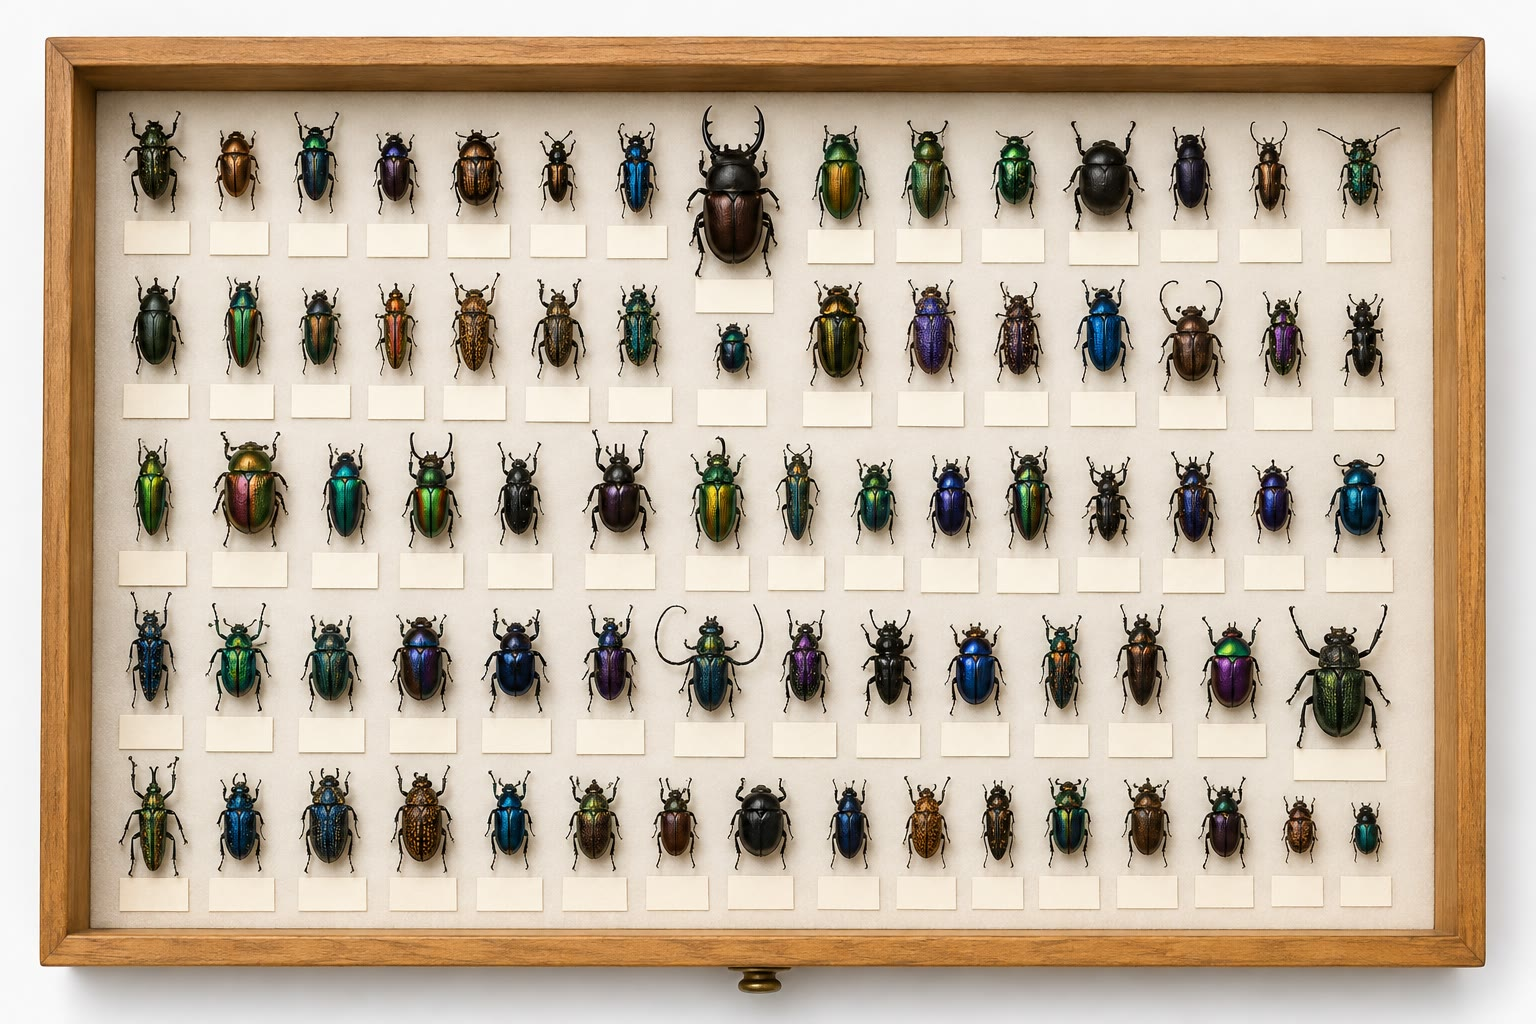
\includegraphics[width=0.56\linewidth]{images/book3/ai/b3-29-beetle-collection.jpg}

{\small 博物馆中一个陈列别针固定甲虫标本的抽屉：馆藏即为
清单，而像这样的抽屉可能容纳尚无人命名的
\omterm{def:b1:classifying-biodiversity:species}{物种}。}
\end{omfigure}

\begin{method}[估算物种总数]\label{met:b1:classifying-biodiversity:estimate}
\begin{enumerate}
  \item 统计某一类群中已描述的\omterm{def:b1:classifying-biodiversity:species}{物种}数，以及
        新\omterm{def:b1:classifying-biodiversity:species}{物种}仍在被加入的速率；若该速率未见放缓，
        则清单远未完整。
  \item 由研究充分的类群按比例外推至研究薄弱的类群：
        若温带动物区系中每一种植物对应两种昆虫，
        而热带有 \num{250000}~种植物，则
        热带至少有五十万种昆虫。
  \item 对小面积区域进行密集取样（以杀虫剂弥雾热带树冠，
        或对一升海水的 \omterm{def:b1:nucleic-acids:chain}{DNA} 进行测序），
        并依据新\omterm{def:b1:classifying-biodiversity:species}{物种}所占的比例向外推算。
  \item 利用各分类阶元之间的规律：门、纲、
        目与科的数目已近乎完整，并向\omterm{def:b1:classifying-biodiversity:species}{物种}水平有规律地增长；
        外推此规律即可得到总数
        （约 870 万种真核生物）。
  \item 估算结果应同时给出其范围；对原核生物而言，
        诚实的答案是一个跨越数个数量级的范围。
\end{enumerate}
\end{method}

\section{练习}

\begin{exercise}[$\star$]\label{exo:b1:classifying-biodiversity:1}
正确写出家猫的学名，指出其属名与种加词，并
将其置于所属的科、目、纲与门之中。
\end{exercise}

\begin{exercise}[$\star$]\label{exo:b1:classifying-biodiversity:2}
定义\omterm{def:b1:classifying-biodiversity:characters}{同源}与趋同，各举一例，并
指出哪一者可作为\omterm{def:b1:classifying-biodiversity:systematics}{演化支}的证据。
\end{exercise}

\begin{exercise}[$\star$]\label{exo:b1:classifying-biodiversity:3}
判断“鱼类”“鸟类”和“温血动物”各自属于
\omterm{def:b1:classifying-biodiversity:monophyly}{单系}、\omterm{def:b1:classifying-biodiversity:monophyly}{并系}还是\omterm{def:b1:classifying-biodiversity:monophyly}{多系}，并说明理由。
\end{exercise}

\begin{exercise}[$\star$]\label{exo:b1:classifying-biodiversity:4}
写出三个域的名称，并给出区分古菌与细菌的
两个特征。
\end{exercise}

\begin{exercise}[$\star\star$]\label{exo:b1:classifying-biodiversity:5}
为何\omterm{def:b1:classifying-biodiversity:species}{生物学物种概念}不能应用于细菌或
化石，代之以何种概念？
\end{exercise}

\begin{exercise}[$\star\star$]\label{exo:b1:classifying-biodiversity:6}
三个\omterm{def:b1:classifying-biodiversity:nomenclature}{分类单元} X、Y、Z 与一个\omterm{def:b1:classifying-biodiversity:characters}{外群}。\omterm{def:b1:classifying-biodiversity:characters}{性状} 1 在 X 和 Y 中为衍生状态；
\omterm{def:b1:classifying-biodiversity:characters}{性状} 2 在 Y 和 Z 中为衍生状态；\omterm{def:b1:classifying-biodiversity:characters}{性状} 3 在 X 和 Y 中为衍生状态；\omterm{def:b1:classifying-biodiversity:characters}{性状} 4 在 X 和
Y 中为衍生状态。画出两种可能的树，计算其\omterm{def:b1:classifying-biodiversity:parsimony}{树长}，并给出
最简约的树及其趋同度。
\end{exercise}

\begin{exercise}[$\star\star$]\label{exo:b1:classifying-biodiversity:7}
构建分支图为何需要\omterm{def:b1:classifying-biodiversity:characters}{外群}，
若所选\omterm{def:b1:classifying-biodiversity:characters}{外群}实际上属于该类群内部，会出现什么问题？
\end{exercise}

\begin{exercise}[$\star\star$]\label{exo:b1:classifying-biodiversity:8}
解释为何动物与真菌被认为比动物与植物
有更近的亲缘关系，并指出后鞭毛生物共有的\omterm{def:b1:classifying-biodiversity:characters}{性状}。
\end{exercise}

\begin{exercise}[$\star\star$]\label{exo:b1:classifying-biodiversity:9}
Woese 发现，产甲烷菌与其他细菌的差异，
与其同真核生物的差异一样大。为何这一发现
足以支持设立新的域，而非仅在细菌之内设立新的界？
\end{exercise}

\begin{exercise}[$\star\star\star$]\label{exo:b1:classifying-biodiversity:10}
用杀虫剂弥雾的一片热带树冠可得到 1200 种甲虫，
其中 \qty{20}{\%} 为该树种所特有；
甲虫占该树冠昆虫的 \qty{40}{\%}，而该树冠
拥有该树昆虫的三分之二；热带树种共有 \num{50000}~种。
估算热带昆虫的\omterm{def:b1:classifying-biodiversity:species}{物种}数，
并列出所用的假设。
\end{exercise}

\begin{exercise}[$\star\star\star$]\label{exo:b1:classifying-biodiversity:11}
某一\omterm{def:b1:classifying-biodiversity:species}{物种}仅依据一份博物馆标本被描述；后来发现了
略有差异的活体\omterm{def:b1:populations:population}{种群}。试说明\omterm{def:b1:classifying-biodiversity:nomenclature}{模式标本}在确定名称适用
范围中的作用，以及优先权为何
重要。
\end{exercise}

\begin{exercise}[$\star\star\star$]\label{exo:b1:classifying-biodiversity:12}
“简约法假定演化走最短路径。”试讨论：
简约法假定了什么，它在何时失效（趋同、快速演化
的谱系），以及如何利用分子数据和化石检验
一棵树。
\end{exercise}

\section{问题：八种脊椎动物与一棵树}

\begin{problem}[{周末问题——八种脊椎动物的性状矩阵，
手工构建其分支图，对两棵相争的树用简约法评分，
检验传统类群的单系性，以及
物种数估计，最后确定最简约的树及其
长度}]
\label{pb:b1:classifying-biodiversity:1}
矩阵对十个\omterm{def:b1:classifying-biodiversity:characters}{性状}评分（1 表示存在衍生状态），类群为
七鳃鳗（\omterm{def:b1:classifying-biodiversity:characters}{外群}）、鲨鱼、鳟鱼、肺鱼、青蛙、蜥蜴、
小鼠和鸽子。

\begin{center}
\footnotesize
\begin{tabular}{l*{10}{c}}
\hline
 & 1 & 2 & 3 & 4 & 5 & 6 & 7 & 8 & 9 & 10 \\
 & \rotatebox{90}{颌} & \rotatebox{90}{硬\omterm{def:b1:body-plans-tissues:segments}{骨骼}} & \rotatebox{90}{肺} & \rotatebox{90}{四肢} & \rotatebox{90}{羊膜卵} & \rotatebox{90}{毛} & \rotatebox{90}{羽毛} & \rotatebox{90}{双孔颅} & \rotatebox{90}{恒温} & \rotatebox{90}{角质鳞片} \\
\hline
七鳃鳗 & 0 & 0 & 0 & 0 & 0 & 0 & 0 & 0 & 0 & 0 \\
鲨鱼 & 1 & 0 & 0 & 0 & 0 & 0 & 0 & 0 & 0 & 0 \\
鳟鱼 & 1 & 1 & 0 & 0 & 0 & 0 & 0 & 0 & 0 & 0 \\
肺鱼 & 1 & 1 & 1 & 0 & 0 & 0 & 0 & 0 & 0 & 0 \\
青蛙 & 1 & 1 & 1 & 1 & 0 & 0 & 0 & 0 & 0 & 0 \\
蜥蜴 & 1 & 1 & 1 & 1 & 1 & 0 & 0 & 1 & 0 & 1 \\
小鼠 & 1 & 1 & 1 & 1 & 1 & 1 & 0 & 0 & 1 & 0 \\
鸽子 & 1 & 1 & 1 & 1 & 1 & 0 & 1 & 1 & 1 & 1 \\
\hline
\end{tabular}
\end{center}

\medskip
\noindent\textbf{第一部分——读取矩阵。}
\begin{enumerate}
  \item 除\omterm{def:b1:classifying-biodiversity:characters}{外群}外，哪些\omterm{def:b1:classifying-biodiversity:characters}{性状}为所有类群所共有？
        它们对这棵树说明了什么？
  \item 按共有衍生状态的类群数目，将\omterm{def:b1:classifying-biodiversity:characters}{性状}排序，
        并说明每个\omterm{def:b1:classifying-biodiversity:characters}{性状}确定了哪个\omterm{def:b1:classifying-biodiversity:systematics}{演化支}。
  \item 哪些\omterm{def:b1:classifying-biodiversity:characters}{性状}只见于单一类群？这些\omterm{def:b1:classifying-biodiversity:characters}{性状}对
        确定该类群的位置是否有用？
  \item 哪一对\omterm{def:b1:classifying-biodiversity:characters}{性状}相互冲突，
        涉及其中哪三个类群？
  \item 给出\omterm{def:b1:classifying-biodiversity:characters}{性状} 3（肺）的极性，
        并说明\omterm{def:b1:classifying-biodiversity:characters}{外群}如何确定该极性。
  \item 其余部分确定后，三种羊膜动物之间可构成
        多少棵不同的有根树？
        哪些\omterm{def:b1:classifying-biodiversity:characters}{性状}与这一选择有关？
\end{enumerate}

\medskip
\noindent\textbf{第二部分——构建树。}
\begin{enumerate}[resume]
  \item 画出由\omterm{def:b1:classifying-biodiversity:characters}{性状} 1 至 5 所隐含的分支图：嵌套的
        \omterm{def:b1:classifying-biodiversity:systematics}{演化支}，从颌一直到羊膜卵。
  \item 在羊膜动物内部，画出树 A（蜥蜴与鸽子
        为姐妹类群）和树 B（小鼠与鸽子
        为姐妹类群）。
  \item 计算树 A 的长度：对十个\omterm{def:b1:classifying-biodiversity:characters}{性状}中的每一个，
        求其所需的最少变化次数。
  \item 同样计算树 B 的长度。
  \item 哪棵树最简约？两者相差多少？
  \item 指出较优的树上的\omterm{def:b1:classifying-biodiversity:characters}{同塑}\omterm{def:b1:classifying-biodiversity:characters}{性状}，
        并说明其演化解释。
  \item 若去掉\omterm{def:b1:classifying-biodiversity:characters}{性状} 8 和 10，两棵树的长度
        各为多少？由此可得出什么结论？
\end{enumerate}

\medskip
\noindent\textbf{第三部分——树上的类群。}
\begin{enumerate}[resume]
  \item 在较优的树上，类群（鲨鱼、鳟鱼、肺鱼）
——即“鱼”——是否为\omterm{def:b1:classifying-biodiversity:monophyly}{单系}？要使其为\omterm{def:b1:classifying-biodiversity:monophyly}{单系}，
        还需加入哪个类群？
  \item 羊膜动物（蜥蜴、小鼠、鸽子）是否为\omterm{def:b1:classifying-biodiversity:monophyly}{单系}？
        试指出其\omterm{def:b1:classifying-biodiversity:characters}{共有衍征}。
  \item 由蜥蜴加上鳄类和龟类组成的类群——即
        传统的“爬行动物”——放入鸽子后是否为\omterm{def:b1:classifying-biodiversity:monophyly}{单系}？
        它属于哪种类群？
  \item 以恒温性归并的（小鼠、鸽子）是否为\omterm{def:b1:classifying-biodiversity:systematics}{演化支}？
        它属于哪一种类群？
  \item 肺鱼常被称为鱼。在这棵树上，它与鳟鱼
        还是与青蛙更近？由哪个\omterm{def:b1:classifying-biodiversity:characters}{性状}决定？
  \item 给出三种羊膜动物在林奈分类中应占的阶元，
        并说明这些阶元为何不能反映
        其分支的深浅。
\end{enumerate}

\medskip
\noindent\textbf{第四部分——\omterm{def:b1:classifying-biodiversity:species}{物种}清单。}
\begin{enumerate}[resume]
  \item 已有约 \num{70000} 种脊椎动物被描述，
        新增描述速率为：鱼类每年 \num{300} 种，
        哺乳动物每年 \num{20} 种。哪一份清单更接近完成？
  \item 对 \qty{1}{L} 海水中的 \omterm{def:b1:nucleic-acids:chain}{DNA} 所作的调查发现
        \num{2000} 条不同的\omterm{def:b1:gene-expression:ribosome}{核糖体}序列，其中
        \qty{90}{\%} 与任何已描述的\omterm{def:b1:organism-environment:organism}{生物体}都不匹配。这对原核生物
        清单意味着什么？
  \item 若背景\omterm{def:b1:classifying-biodiversity:biodiversity}{灭绝}速率为每年每百万\omterm{def:b1:classifying-biodiversity:species}{物种}\omterm{def:b1:classifying-biodiversity:biodiversity}{灭绝}一种，
        真核生物约有 900 万种，则每年应有多少种\omterm{def:b1:classifying-biodiversity:biodiversity}{灭绝}？
        已观察到的研究较充分类群的\omterm{def:b1:classifying-biodiversity:biodiversity}{灭绝}速率
        约高 \num{1000} 倍。由此，所有真核生物每年
        \omterm{def:b1:classifying-biodiversity:biodiversity}{灭绝}多少种？
  \item 为何在被描述之前即已\omterm{def:b1:classifying-biodiversity:biodiversity}{灭绝}的\omterm{def:b1:classifying-biodiversity:species}{物种}，
        对\omterm{def:b1:classifying-biodiversity:systematics}{系统学}和\omterm{def:b1:ecosystem-organization:ecosystem}{生态系统}都是损失？
  \item 说明为何已描述的科数比已描述的\omterm{def:b1:classifying-biodiversity:species}{物种}数
        更能反映总数？
  \item 给出结果：八种脊椎动物中最简约的树，
        以嵌套括号表示，并给出其长度。
\end{enumerate}
\end{problem}
